\begin{frame}
    \begin{listing}[H]
        \inputsource[fontsize=\fontsize{9}{9}, firstline=41, lastline=64]{py}{tflite/tflite_sinewave_training.py}
        \caption{Generate random samples.}
        \label{lst:tflite:sinewave:generate_samples}
    \end{listing}
\end{frame}

\begin{frame}
    \begin{figure}
        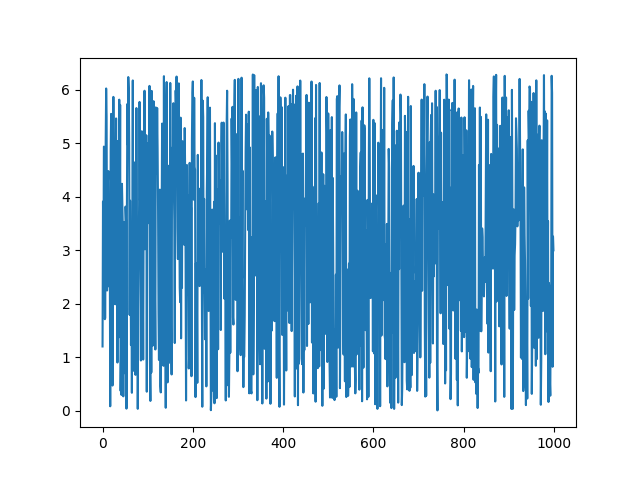
\includegraphics[width=0.85\textwidth]{images/tflite/colab/x-values.png}
        \caption{Random samples (x values).}
    \end{figure}
\end{frame}

\begin{frame}
    \begin{figure}
        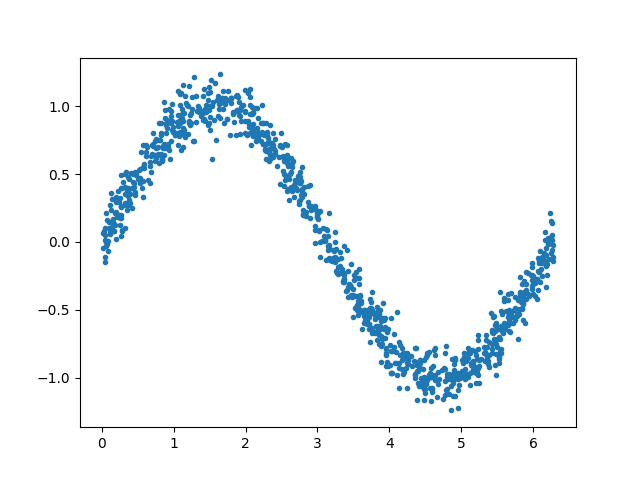
\includegraphics[width=0.85\textwidth]{images/tflite/colab/y-values.png}
        \caption{Random samples (y values).}
    \end{figure}
\end{frame}

\begin{frame}
    \begin{figure}
        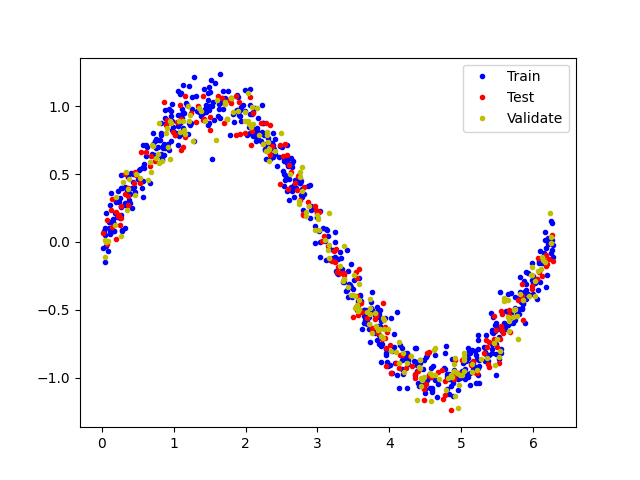
\includegraphics[width=0.85\textwidth]{images/tflite/colab/sets.png}
        \caption{Random sample sets: training, validation, test.}
    \end{figure}
\end{frame}